\subsection{Game V3}
The game rules of Game V3 provide a slight advantage to the prey as if the prey run off of the board, then the predator's score decreases as they could not catch the prey. However, this rule should prevent the patrolling behaviour that was developed in Game V2. Using these rules, most of the predator experiments had trouble reaching a fitness value of -1, while only a couple of runs reached a fitness value of -0.75 (see Figures \ref{fig:v3-pred-runs} and \ref{fig:v3-pred-runs-2}). The prey on the other hand improved significantly from game V2. The prey fitness with these game rules hovers close to 1 with the fitness only going below 0.75 on rare occasion. 


\begin{figure}
  \centering
  \begin{subfigure}{0.7\textwidth}
    \centering
    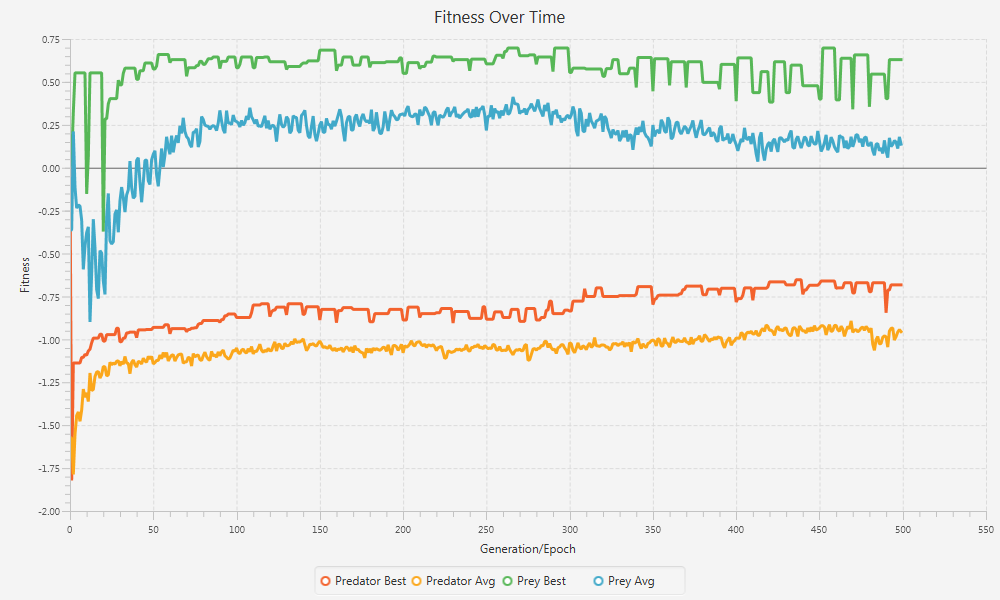
\includegraphics[width=\linewidth]{v3-exp26-Run-4.png}
    \caption{Experiment 2 Run 5}
  \end{subfigure}
  \begin{subfigure}{0.7\textwidth}
    \centering
    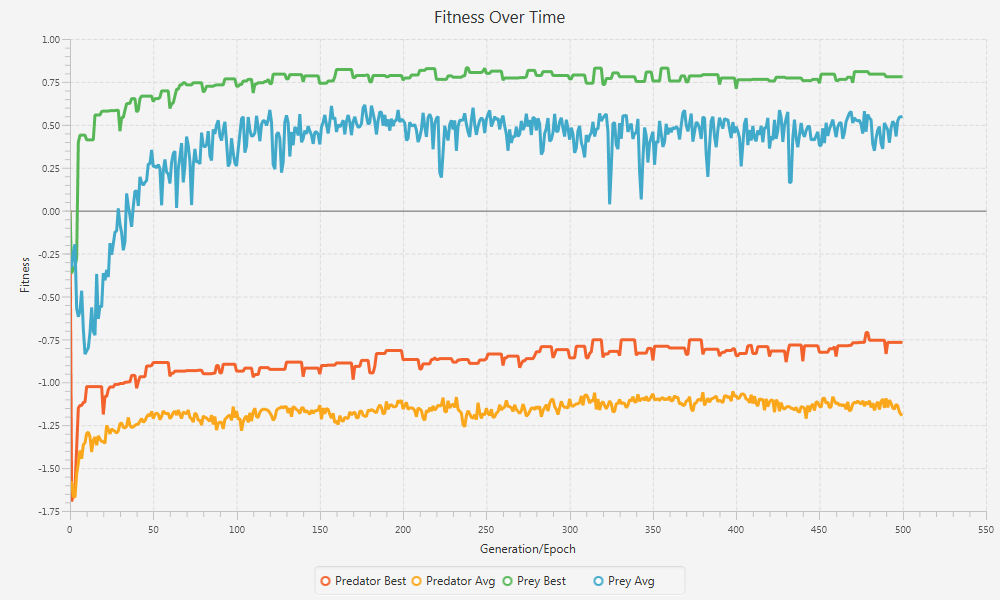
\includegraphics[width=\linewidth]{v3-exp27-Run-3.png}
    \caption{Experiment 3 Run 4}
  \end{subfigure}
    \caption{Game V3 fitness over time examples above -0.75\label{fig:v3-pred-runs}}
\end{figure}




\begin{figure}
  \centering
    \begin{subfigure}{0.7\textwidth}
    \centering
    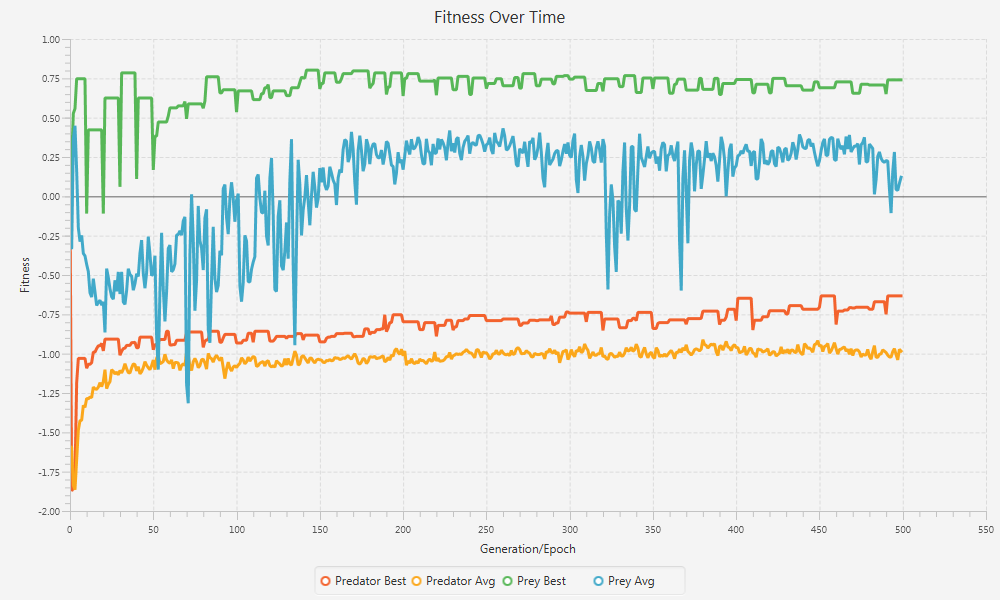
\includegraphics[width=\linewidth]{v3-exp47-Run-2.png}
    \caption{Experiment 23 Run 3}
  \end{subfigure}
  \begin{subfigure}{0.7\textwidth}
    \centering
    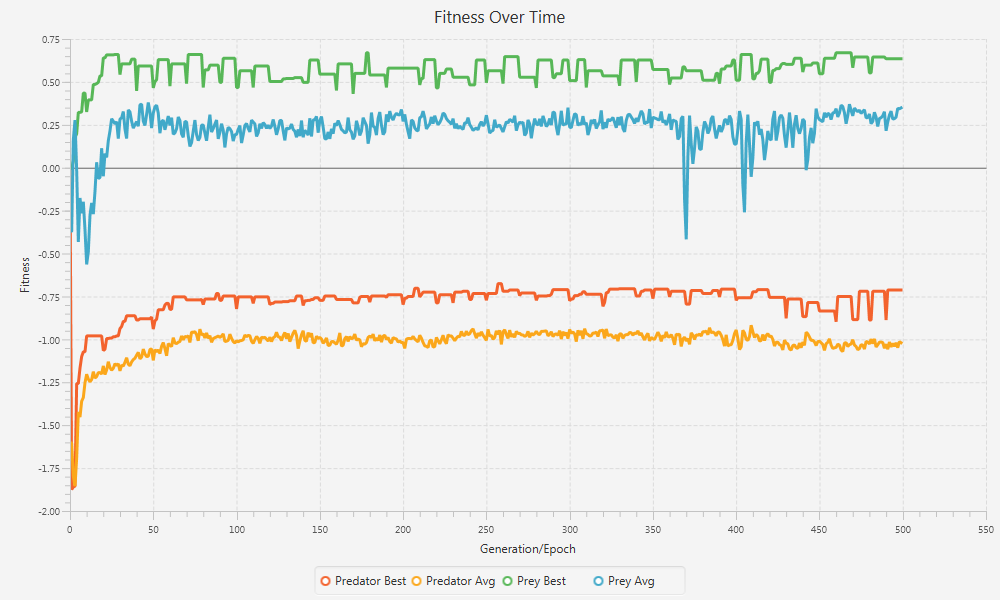
\includegraphics[width=\linewidth]{v3-exp47-Run-4.png}
    \caption{Experiment 23 Run 5}
  \end{subfigure}
  \caption{Game V3 fitness over time examples above -0.75 continued\label{fig:v3-pred-runs-2}}
\end{figure}

\begin{figure}
  \centering
  \begin{subfigure}{0.4\textwidth}
    \centering
    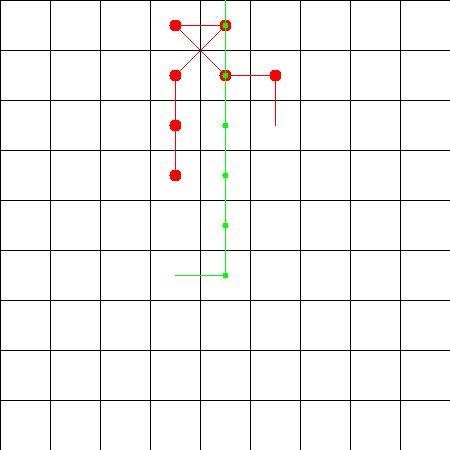
\includegraphics[width=\linewidth]{v3-exp47-r4-Game-24.png}
    \caption{Game 24}
  \end{subfigure}
  \begin{subfigure}{0.4\textwidth}
    \centering
    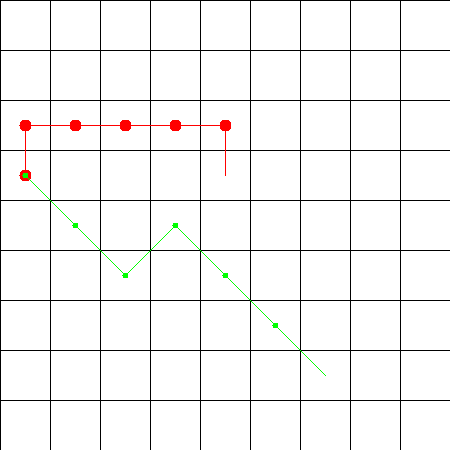
\includegraphics[width=\linewidth]{v3-exp47-r4-Game-33.png}
    \caption{Game 33}
  \end{subfigure} \\\hfill
  
  \begin{subfigure}{0.4\textwidth}
    \centering
    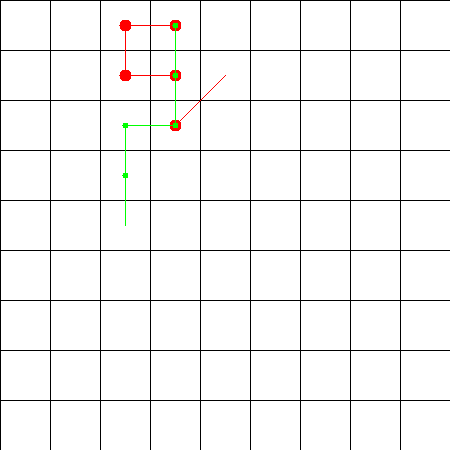
\includegraphics[width=\linewidth]{v3-exp47-r4-Game-45.png}
    \caption{Game 45}
  \end{subfigure}
  \begin{subfigure}{0.4\textwidth}
    \centering
    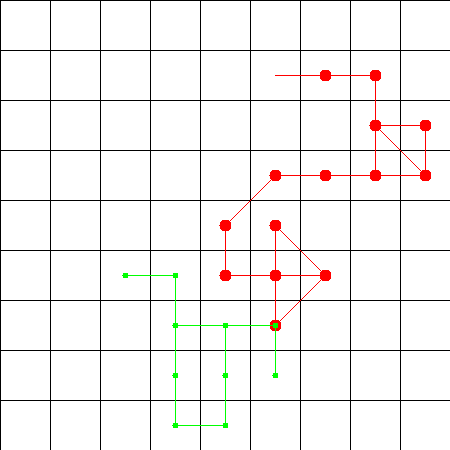
\includegraphics[width=\linewidth]{v3-exp47-r4-interesting-Game-91.png}
    \caption{Game 91}
  \end{subfigure}
  \caption{Game V3 Experiment 23 Run 5: Predator Game Examples\label{fig:v3-pred-best-games}}
\end{figure}


\begin{figure}
  \centering
  \begin{subfigure}{0.4\textwidth}
    \centering
    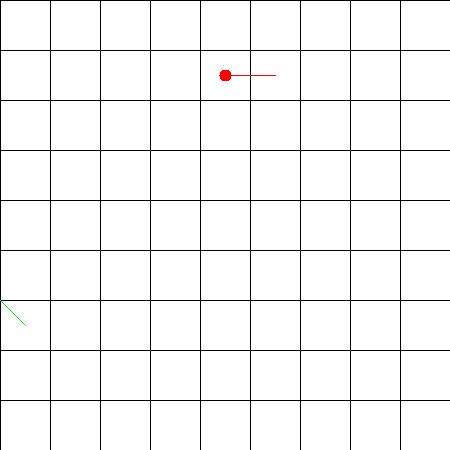
\includegraphics[width=\linewidth]{v3-exp47-r4-1-Game-327.png}
    \caption{Game 327}
  \end{subfigure}
  \begin{subfigure}{0.4\textwidth}
    \centering
    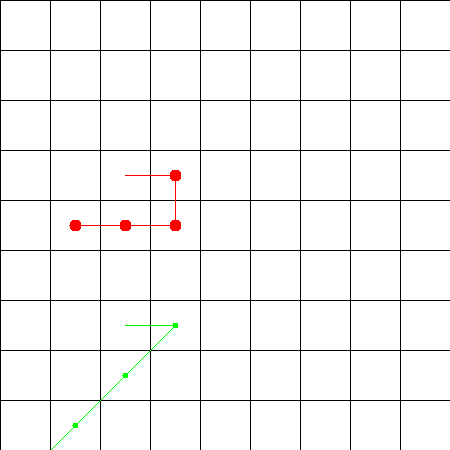
\includegraphics[width=\linewidth]{v3-exp47-r4-1-Game-328.png}
    \caption{Game 328}
  \end{subfigure} \\\hfill
  
  \begin{subfigure}{0.4\textwidth}
    \centering
    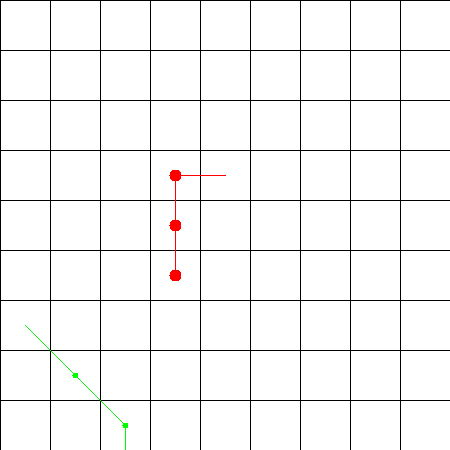
\includegraphics[width=\linewidth]{v3-exp47-r4-1-Game-329.png}
    \caption{Game 329}
  \end{subfigure}
  \begin{subfigure}{0.4\textwidth}
    \centering
    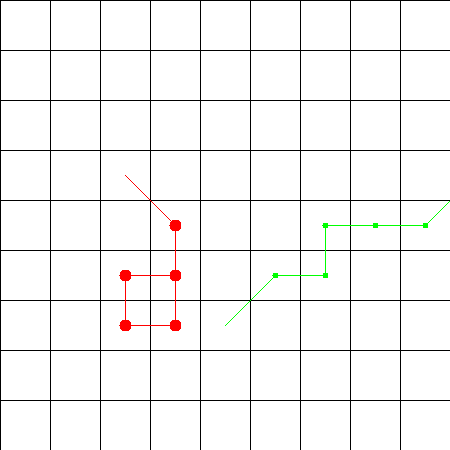
\includegraphics[width=\linewidth]{v3-exp47-r4-1-Game-330.png}
    \caption{Game 330}
  \end{subfigure}
  \caption{Game V3 Experiment 23 Run 5: Prey Running off of the Board Examples\label{fig:v3-prey-running-off-board}}
\end{figure}


As it can be seen, experiment 23 seems to provide the best results for this set of game rules for the predator as there are two instances where the best fitness surpasses -0.75. Some games played with complex behaviour in experiment 23 run 4 can be seen in Figure \ref{fig:v3-pred-best-games}. While the predator is not the best at catching the prey, in some games, complex patterns start to emerge. Unfortunately and interestingly most games end with the prey leaving the board (examples in Figure \ref{fig:v3-prey-running-off-board}). This could be due to the fact that the prey is exploiting the rules of game V3. By leaving the board, the prey can be at a net difference in fitness of -1, however if the predator succeeds in catching the prey, then the prey would be at a net different of -2, therefore it is more beneficial for the prey if it runs off the board. Therefore, the change in game rules that was added to try to motivate the predator to capture the prey was in turn used against the predator. It can also be seen that even when the prey is in the process of running off the board, the predator is approaching the prey, which is consistent with the walled game.



It should be noted that in all graphs in Figure \ref{fig:v3-pred-runs}, the prey average converges slower to the prey best. This seems to suggest that having most of the population be poor in the beginning provides an advantage to the prey to prevent the predators from learning. Comparing the way the prey converges to the graphs in Figure \ref{fig:v2-pred-better-graphs} this is even more evident.



\begin{table}
  \centering
  \begin{tabular}{|c|c|c|c|c|c|c|}
    \hline
    \multirow{2}{*}{Experiment} & \multicolumn{3}{|c|}{Predator} & \multicolumn{3}{|c|}{Prey} \\\cline{2-7}
    & Max & Average & Min & Max & Average & Min\\
    \hline
    1 & -0.755 & -0.866 & -0.923 & 0.817 & 0.798 & 0.745 \\
2 & -0.653 & -0.850 & -0.975 & 0.885 & 0.690 & 0.412 \\
3 & -0.710 & -0.846 & -0.893 & 0.766 & 0.612 & 0.520 \\
4 & -0.903 & -0.920 & -0.940 & 0.821 & 0.674 & 0.580 \\
5 & -0.803 & -0.894 & -0.958 & 0.898 & 0.816 & 0.648 \\
6 & -0.788 & -0.873 & -0.955 & 0.777 & 0.699 & 0.562 \\
7 & -0.783 & -0.821 & -0.900 & 0.732 & 0.548 & 0.395 \\
8 & -0.753 & -0.889 & -0.943 & 0.844 & 0.788 & 0.670 \\
9 & -0.833 & -0.900 & -0.948 & 0.887 & 0.775 & 0.637 \\
10 & -0.785 & -0.893 & -0.940 & 0.899 & 0.761 & 0.547 \\
11 & -0.773 & -0.848 & -0.940 & 0.859 & 0.657 & 0.509 \\
12 & -0.858 & -0.869 & -0.885 & 0.746 & 0.640 & 0.467 \\
13 & -0.868 & -0.919 & -0.968 & 0.843 & 0.819 & 0.735 \\
14 & -0.718 & -0.879 & -0.963 & 0.868 & 0.754 & 0.604 \\
15 & -0.850 & -0.889 & -0.925 & 0.831 & 0.766 & 0.688 \\
16 & -0.888 & -0.910 & -0.933 & 0.842 & 0.732 & 0.573 \\
17 & -0.665 & -0.816 & -0.920 & 0.897 & 0.770 & 0.649 \\
18 & -0.903 & -0.929 & -0.955 & 0.867 & 0.779 & 0.729 \\
19 & -0.883 & -0.900 & -0.928 & 0.856 & 0.774 & 0.649 \\
20 & -0.763 & -0.862 & -0.905 & 0.824 & 0.708 & 0.498 \\
21 & -0.735 & -0.877 & -0.935 & 0.856 & 0.762 & 0.492 \\
22 & -0.835 & -0.892 & -0.953 & 0.884 & 0.722 & 0.595 \\
23 & -0.633 & -0.782 & -0.900 & 0.787 & 0.584 & 0.380 \\
24 & -0.818 & -0.925 & -0.993 & 0.852 & 0.710 & 0.417 \\

    \hline
  \end{tabular}
  \caption{Game V3 Summary}
  \label{tab:v3-summary}
\end{table}

In Table \ref{tab:v3-summary}, the prey tends to have higher average results when comparing 0\% charged swarms to 100\% charged swarms. This is because the prey's fitness is much better than the predators, so there is no need to explore more of the error landscape. Interestingly, the predator also follows this pattern even though exploring the error landscape should lead to better solutions.